% -----------------------------------------------
% Template for SMAC SMC 2013
% adapted and corrected from the template for SMC 2012, which was adapted from that of SMC 2011
% further updated for TENOR 2015 and 2016
% -----------------------------------------------

\documentclass{article}
\usepackage{tenor2016}
%\usepackage{times}
\usepackage{ifpdf}
\usepackage[english]{babel}
%\usepackage{cite}

%%%%%%%%%%%%%%%%%%%%%%%% Some useful packages %%%%%%%%%%%%%%%%%%%%%%%%%%%%%%%
%%%%%%%%%%%%%%%%%%%%%%%% See related documentation %%%%%%%%%%%%%%%%%%%%%%%%%%
%\usepackage{amsmath} % popular packages from Am. Math. Soc. Please use the 
%\usepackage{amssymb} % related math environments (split, subequation, cases,
%\usepackage{amsfonts}% multline, etc.)
%\usepackage{bm}      % Bold Math package, defines the command \bf{}
%\usepackage{paralist}% extended list environments
%%subfig.sty is the modern replacement for subfigure.sty. However, subfig.sty 
%%requires and automatically loads caption.sty which overrides class handling 
%%of captions. To prevent this problem, preload caption.sty with caption=false 
%\usepackage[caption=false]{caption}
%\usepackage[font=footnotesize]{subfig}


%user defined variables
\def\papertitle{Symbolic scores as dynamic expressions}
\def\firstauthor{Gabriel Lepetit-Aimon}
\def\secondauthor{Dominique Fober}
\def\thirdauthor{Third author}

% adds the automatic
% Saves a lot of ouptut space in PDF... after conversion with the distiller
% Delete if you cannot get PS fonts working on your system.

% pdf-tex settings: detect automatically if run by latex or pdflatex
\newif\ifpdf
\ifx\pdfoutput\relax
\else
   \ifcase\pdfoutput
      \pdffalse
   \else
      \pdftrue
\fi

\ifpdf % compiling with pdflatex
  \usepackage[pdftex,
    pdftitle={\papertitle},
    pdfauthor={\firstauthor, \secondauthor, \thirdauthor},
    bookmarksnumbered, % use section numbers with bookmarks
    pdfstartview=XYZ % start with zoom=100% instead of full screen; 
                     % especially useful if working with a big screen :-)
   ]{hyperref}
  %\pdfcompresslevel=9

  \usepackage[pdftex]{graphicx}
  % declare the path(s) where your graphic files are and their extensions so 
  %you won't have to specify these with every instance of \includegraphics
  \graphicspath{{./figures/}}
  \DeclareGraphicsExtensions{.pdf,.jpeg,.png}

  \usepackage[figure,table]{hypcap}

\else % compiling with latex
  \usepackage[dvips,
    bookmarksnumbered, % use section numbers with bookmarks
    pdfstartview=XYZ % start with zoom=100% instead of full screen
  ]{hyperref}  % hyperrefs are active in the pdf file after conversion

  \usepackage[dvips]{epsfig,graphicx}
  % declare the path(s) where your graphic files are and their extensions so 
  %you won't have to specify these with every instance of \includegraphics
  \graphicspath{{./figures/}}
  \DeclareGraphicsExtensions{.eps}

  \usepackage[figure,table]{hypcap}
\fi

%setup the hyperref package - make the links black without a surrounding frame
\hypersetup{
    colorlinks,%
    citecolor=black,%
    filecolor=black,%
    linkcolor=black,%
    urlcolor=black
}


% Title.
% ------
\title{\papertitle}

% Authors
% Please note that submissions are NOT anonymous, therefore 
% authors' names have to be VISIBLE in your manuscript. 
%
% Single address
% To use with only one author or several with the same address
% ---------------
%\oneauthor
%   {\firstauthor} {Affiliation1 \\ %
%     {\tt \href{mailto:author1@adomain.org}{author1@adomain.org}}}

%Two addresses
%--------------
 \twoauthors
   {\firstauthor} {Grame \\ %
     {\tt \href{mailto:gabriel.lepetit.aimon@grame.fr}{gabriel.lepetit.aimon@grame.fr}}}
   {\secondauthor} {Grame \\ %
     {\tt \href{mailto:fober@grame.fr}{fober@grame.fr}}}

% Three addresses
% --------------
% \threeauthors
%   {\firstauthor} {Affiliation1 \\ %
%     {\tt \href{mailto:author1@adomain.org}{author1@adomain.org}}}
%   {\secondauthor} {Affiliation2 \\ %
%     {\tt \href{mailto:author2@adomain.org}{author2@adomain.org}}}
%   {\thirdauthor} { Affiliation3 \\ %
%     {\tt \href{mailto:author3@adomain.org}{author3@adomain.org}}}


% ***************************************** the document starts here ***************
\begin{document}
%
\capstartfalse
\maketitle
\capstarttrue
%
\begin{abstract}
Place your abstract at the top left column on the first page.
Please write about 150-200 words that specifically highlight the purpose of your work,
its context, and provide a brief synopsis of your results.
Avoid equations in this part.
\end{abstract}
%

\section{Introduction}\label{sec:introduction}



\section{Page size and format}\label{sec:page_size}
Your paper must not exceed {\bf 12 pages},
no matter if you are presenting orally or posterly.
We \underline{strongly encourage}
a paper length of {\bf 6 pages}.
We will format the proceedings as
 \underline{portrait A4-size paper} \underline{(21.0~cm x 29.7~cm)}.
All material on each page should fit within a rectangle of 17.2~cm x 25.2~cm,
centered on the page, beginning 2.0~cm from the top of the page and ending 
with 2.5cm from the bottom.
The left and right margins should be 1.9~cm.
The text should be in two 8.2~cm columns with a 0.8~cm gutter.
All text must be in a two-column format, and justified.
If you prepare your document by cutting and pasting into this one,
then you should not have to worry, 
unless there is something strange with your \LaTeX{} interpreter.
So double check.
If you have any questions, please contact the TENOR 2016 Organizers.

\section{Typeset Text}\label{sec:typeset_text}

\subsection{Normal or Body Text}\label{subsec:body}
Please use a 10pt (point) Times font. 
Use sans-serif or non-proportional fonts
only for special purposes, 
such as distinguishing source code.
The first paragraph in each section should not be indented, 
but all other paragraphs should be.

\subsection{Title and Authors}
As you can see above, the title is 16pt Times, bold, upper case, and centered.
The names of the authors are also centered.
The lead author's name is to be listed first (left-most), and the co-authors' 
names after. If the addresses for all authors are the same, include the 
address only once, centered. If the authors have different addresses, put the 
addresses, evenly spaced, under each authors' name.

\subsection{First Page Copyright Notice}
Please leave the copyright notice exactly as it appears in the lower 
left-hand corner of the first page. It is set in 8pt Times, if you are wondering.

\subsection{Page Numbering, Headers and Footers}
Do not include headers, footers or page numbers in your submission.
We add these electronically when we assemble the publications
into the proceedings.

\section{Headings}
First level headings are in Times 12pt bold,
centered with 1 line of space above the section head, and 1/2 space below it.
For a section header immediately followed by a subsection header, the space 
should be merged.

\subsection{Second Level Headings}
Second level headings are in Times 10pt bold, flush left,
with 1 line of space above the section head, and 1/2 space below it.
The first letter of each significant word is capitalized.

\subsubsection{Third Level Headings}
Third level headings are in Times 10pt italic, flush left,
with 1/2 line of space above the section head, and 1/2 space below it.
The first letter of significant words is capitalized.

\subsubsection{Level Headings Beyond the Third}
We strongly discourage any use of
more than three levels of headings.
Also, if you have only one subsection in a section,\footnote{Just like this section.}
then you should reorganize it into one section.

\section{Floats and equations}

\subsection{Equations}
Equations of importance, 
or to which you refer later,
should be placed on separated lines and numbered.
The number should be on the right side, in parentheses.
\begin{equation}
E=mc^{2+\delta}.
\label{eq:Emc2}
\end{equation}
Refer to equations like so:
As (\ref{eq:Emc2}) shows, 
I do not completely trust Special Relativity.

\subsection{Figures, Tables and Captions}
\begin{table}[t]
 \begin{center}
 \begin{tabular}{|l|l|}
  \hline
  String value & Numeric value \\
  \hline
  Hello TENOR  & 2016 \\
  \hline
 \end{tabular}
\end{center}
 \caption{Table captions should be placed below the table, exactly like this,
 but using words different from these.}
 \label{tab:example}
\end{table}

All artwork must be centered, neat, clean, and legible.
And if you include figures in your paper, instead of artwork,
please make sure they are centered, neat, clean,
and completely legible without super resolution imaging.
All lines should be thick and dark enough to be reproducible
even by a facsimile machine;
and figures should not be hand-drawn unless your hand is robotically precise.
Since the proceedings are distributed in electronic form only, 
we allow color to be used in figures;
but please check that your figures are 
coherent if they are printed in black-and-white.
For instance, to make your figures zing in several conditions,
vary line thickness, style, and color at the same time.

Numbers and captions of figures and tables always appear below the figure/table.
Leave 1 line space between the figure or table and the caption.
Figure and tables are numbered consecutively. 
Captions should be Times 10pt.
And try to make your captions sufficiently explain your figures and tables.
Place tables/figures in text as close to the reference as possible, 
and preferably at the top of the page.

Always refer to tables and figures in the main text, for example:
see Fig. \ref{fig:example} and \tabref{tab:example}.
Figures and tables may extend across both columns to a maximum width of 17.2cm.

Vectorial figures are preferred, e.g., eps.
When using \texttt{Matlab}, 
export using either (encapsulated) Postscript or PDF format. 
In order to optimize readability, 
the font size of text within a figure should be no smaller than
that of footnotes (8pt font-size). 
If you use bitmap figures, make sure that 
the resolution is high enough for print quality. 

%\begin{figure}[t]
%\centering
%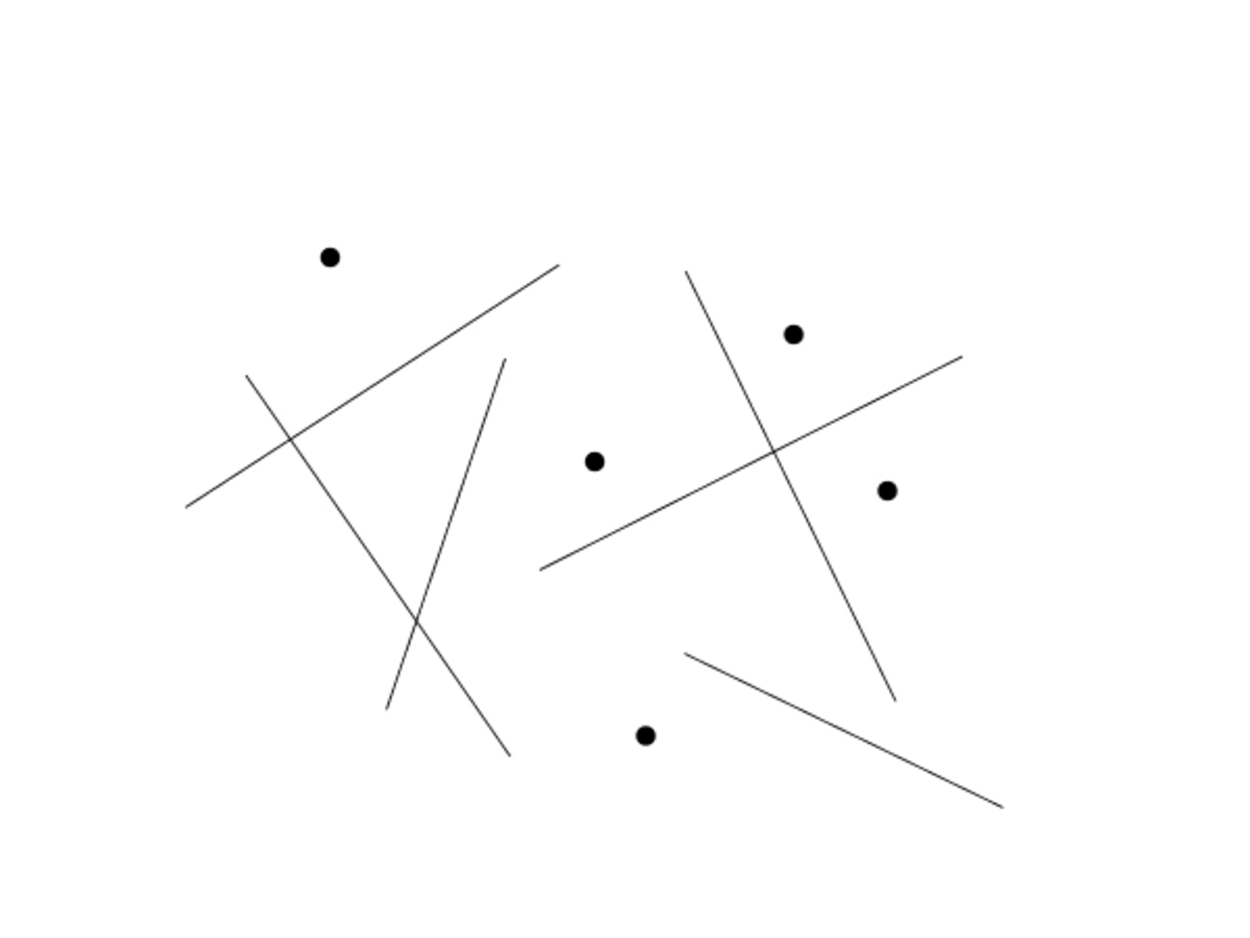
\includegraphics[width=0.9\columnwidth]{figure}
%\caption{Figure captions should be placed below the figure, 
%exactly like this.
%\label{fig:example}}
%\end{figure}

%\begin{figure}[t]
%\figbox{
%\subfloat[][]{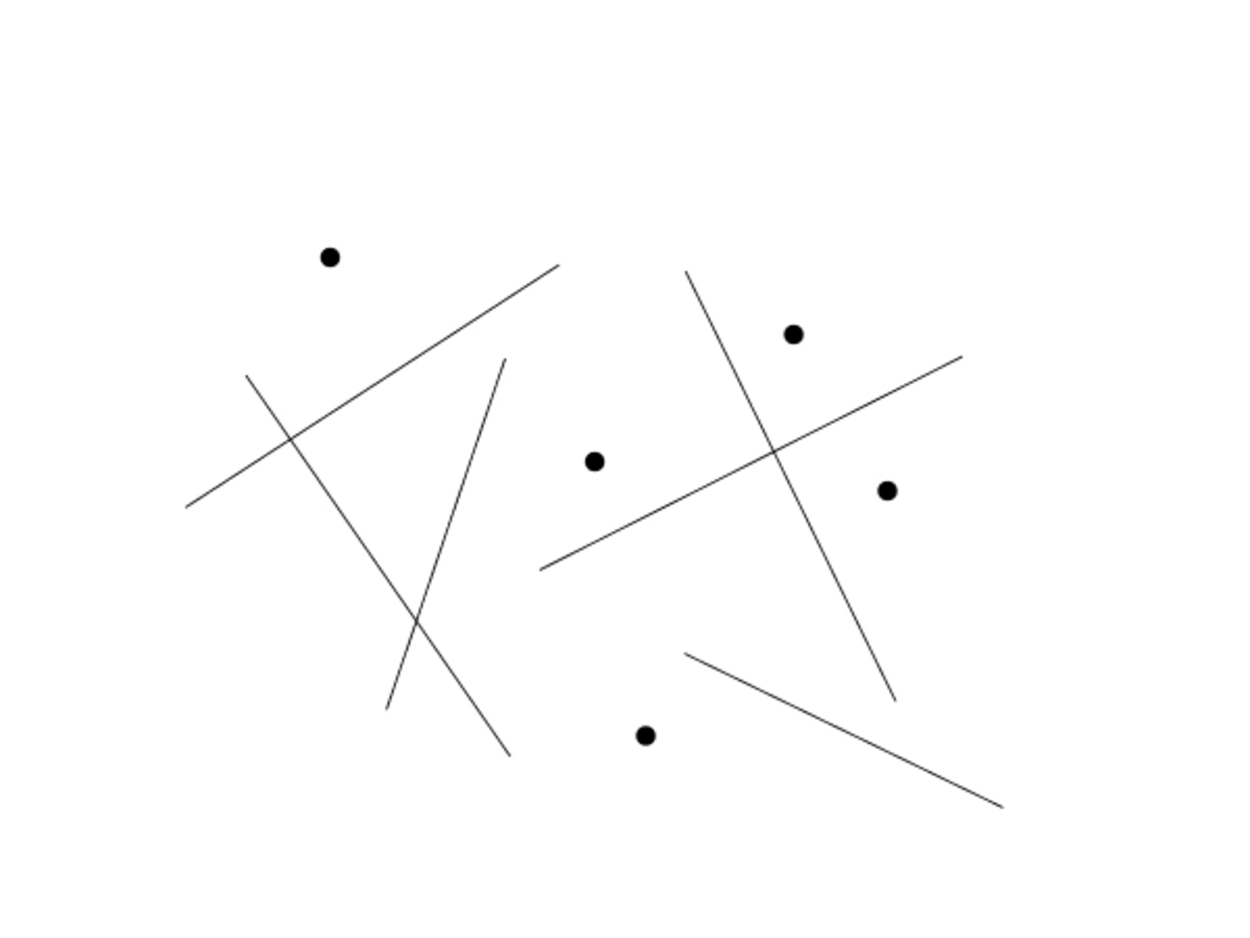
\includegraphics[width=60mm]{figure}\label{fig:subfigex_a}}\\
%\subfloat[][]{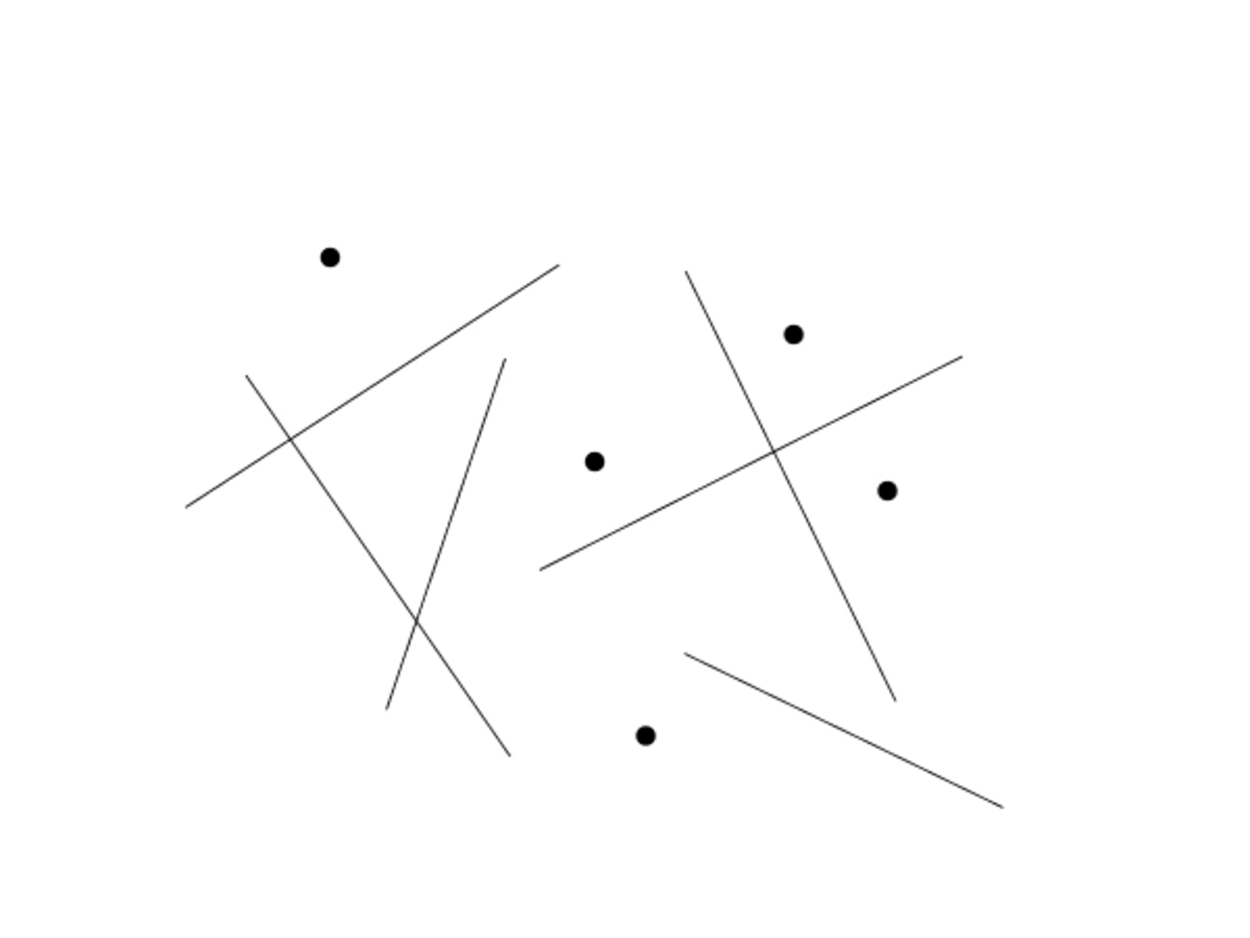
\includegraphics[width=80mm]{figure}\label{fig:subfigex_b}}
%}
%\caption{Here's an example using the subfig package.\label{fig:subfigex} }
%\end{figure}

\subsection{Footnotes}
You can indicate footnotes with a number in the text,\footnote{This is a footnote.}
but try to work the content into the main text.
Use 8pt font-size for footnotes. 
Place the footnotes at the bottom of the page 
on which they appear. 
Precede the footnote with a 0.5pt horizontal rule.

\section{Citations}
List all bibliographical references at the end of your paper,
inside a section named ``REFERENCES''.
Order and number the references in order of appearance. 
Do not list references that do not appear in the text.
Reference numbers in the text should appear within square brackets, such as 
in~\cite{Someone:13} or~\cite{Someone:13,Someone:04,Someone:09}.
The reference format is the standard IEEE one. 
We highly recommend you use BibTeX 
to generate the reference list.

\section{Conclusions}
To finish your full-length paper, end it with a conclusion;
and after careful editing and a final spell-cheek,
submit it through the \href{https://easychair.org/conferences/?conf=tenor2016}{\textcolor {magenta} {\underline {EasyChair Submission System}}}. 
\underline{Do not} send papers directly by e-mail.
%
\begin{acknowledgments}
You may acknowledge people, projects, 
funding agencies, etc. 
which can be included after the second-level heading
``Acknowledgments'' (with no numbering).
\end{acknowledgments} 

%%%%%%%%%%%%%%%%%%%%%%%%%%%%%%%%%%%%%%%%%%%%%%%%%%%%%%%%%%%%%%%%%%%%%%%%%%%%%
%bibliography here
\bibliography{tenor2016template}

\end{document}
